% !TeX root = ../main.tex

\chapter{低维材料简介}

\section{低维材料的基本概念}

所谓\textit{低维材料},即维数小于三的材料,具体来说,分为二维材料、一维材料和零维材料。在某一维上不计维数,通常指在该维方向上材料有纳米尺度($1\sim 100\si{\nano\meter}$)限制。

\begin{itemize}
    \item 二维材料,包括两种材料的界面,或附着在基片上的薄膜,界面的深或膜层的厚度在纳米量级。

    \item 一维材料又称量子线,线的粗细为纳米量级。

    \item 零维材料,又称量子点,由少数原子或分子堆积而成,微粒的大小为纳米量级。
\end{itemize}

\section{低维材料的例子}

首先,我们对于三种维数的低维材料给出例子。

二维材料有半导体量子阱。

一维材料有碳纳米管。

\begin{figure}
    \centering
    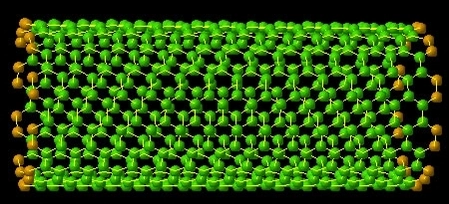
\includegraphics[scale=0.7]{img/碳纳米管}
    \caption{碳纳米管}
\end{figure}

零维材料有半导体和金属的原子簇。

\begin{figure}
    \centering
    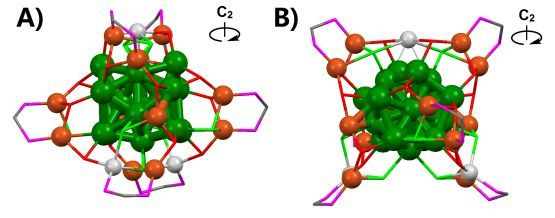
\includegraphics[scale=0.7]{img/金属原子簇}
    \caption{金属原子簇:$\ce{[Ag_{20}Cu_{12}(SR)_{14}(Dppm)_6Br_8]^{2+}}$}
\end{figure}

其次,我们简单介绍一些前沿低维材料。

响应性含硒/碲高分子,可应用于药物可控释放、动态响应\cite{RN41}。

高分子氢键复合物低维材料,可制备功能性的薄膜或涂层。
